\documentclass{beamer}
\usetheme{Darmstadt}
\usepackage{beamerthemesplit}
\usepackage{latexsym}
\usepackage{ae,aecompl}
\usepackage{graphicx}
\usepackage{amsfonts}
\usepackage{tikz}
\usepackage{graphics}
\usepackage{url}

\graphicspath{{../images/}}

\hypersetup{
  pdftitle={MSWL Project Evaluation: OpenNebula Project Analysis},
  pdfauthor={Sergio Arroutbi Braojos},
  pdfcreator={},
  pdfproducer=PDFLaTeX,
  pdfsubject={nn},
}

\title{MSWL Project Evaluation: OpenNebula Project Analysis}
\author{Sergio Arroutbi Braojos}
\begin{document}
% Background Image
\setbeamertemplate{background}{%
    \tikz\node[opacity=0.1] at (current page.center) {
    \vbox to \paperheight{\vfil\hbox to \paperwidth{\hfil
\includegraphics[width=6cm]{opennebula.png}\hfil}\vfil}
 };
}
\frame{\titlepage
\begin{flushright}
{\tiny
(cc) 2014 Sergio Arroutbi Braojos.
    This work is under a license Creative Commons CC-BY 3.0.\\
To view a copy of full license, see \url{http://creativecommons.org/licenses/by/3.0/}
}
\begin{figure}[h]
    \begin{flushright}	
        
\includegraphics[width=0.6in]{by.png}
        \label{fig:by}
    \end{flushright}
\end{figure}
\end{flushright}
}

%\section[Index]{}
%\begin{frame}[allowframebreaks]
%\tableofcontents
%\end{frame}

\section{About}

% Presentation
\begin{frame}[allowframebreaks]
\frametitle{About OpenNebula}

\begin{itemize}
	\item FLOSS Cloud Computing Framework:\linebreak
	- Flexible Enterprise Cloud Made Simple\linebreak
	- Mission: Simple but feature-rich and flexible solution to build and manage enterprise clouds and virtualized data centers\linebreak
 - Main Objective: Lead innovation in enterprise-class cloud data center management\linebreak
 - Core Values: 
   \begin{enumerate}\itemsep0pt
   \item{Openness}
   \item{Excellence}
   \item{Cooperation}
   \item{Innovation}
   \end{enumerate}
	\item Project Start: 2008\\
 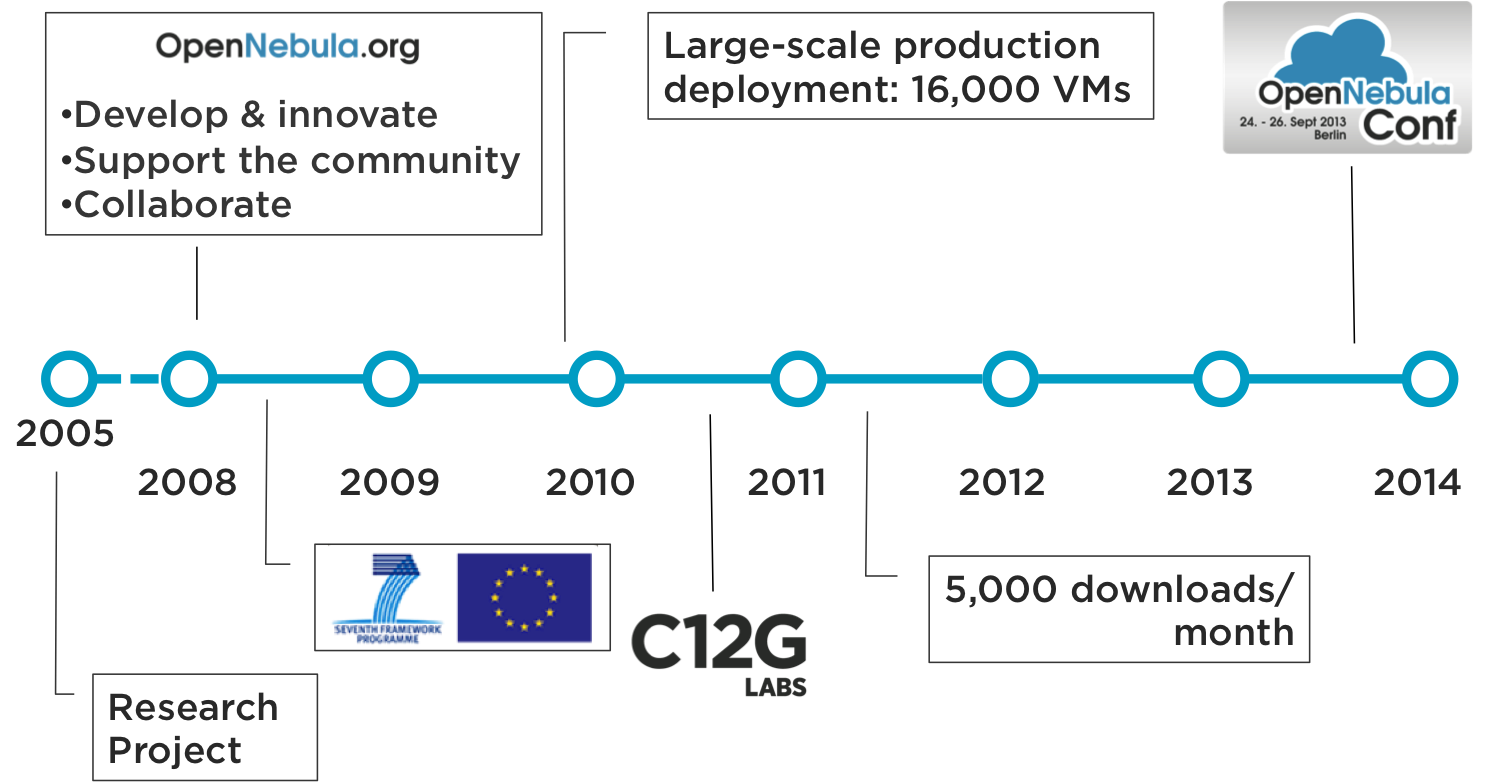
\includegraphics[width=4in]{opennebula-history.png}
\end{itemize}

\end{frame}

\section{Art State}

% Presentation
\begin{frame}[allowframebreaks]
\frametitle{Cloud Computing State of the Art }

\begin{itemize}
	\item OpenNebula \\
	- CG12 Labs, Focused on Functionality, Weak Community
	\item CloudStack \\
	- Open CloudStack, by Apache (Community, Openness)
	\item Eucalyptus \\ 
	- OpenSource AWS Compatible Private Clouds
	\item OpenStack \\
	- More than 200 hundred companies involved
\end{itemize}

\end{frame}

\section{Community}

% Origin
\begin{frame}[allowframebreaks]
\frametitle{Drupal Community}

"Drupal is more than software - it is a project and a community." \linebreak

"So fostering the Drupal community is actually more important than just managing the code base."

 \hfill - Dries Buytaert

\textbf{[ Community ]}

\emph{groups.drupal.org} provides a place for groups to: \\
- organize \\
- meet \\
- work on projects based on interest or geographic location \linebreak

	
Events \& Meetups, Chat (IRC), Planet Drupal, Community Spotlight, Commercial Support, Forum, Mailing Lists, 'Drupal Association'.

\end{frame}


\section{Roles}

% Origin
\begin{frame}[allowframebreaks]
\frametitle{Drupal Main Roles}

\textbf{[ Contributors/Volunteers ]}

    \begin{itemize}
    	\item Code Developing
    	\item Documentation
    	\item Marketing
    	\item User Support
    	\item Testing
    	\item Translation
    	\item ..and a wide range of abilities and interests
	\end{itemize}
\end{frame}


\section{Requirements}

% Origin
\begin{frame}[allowframebreaks]
\frametitle{Candidate's Requirements}

    \begin{itemize}
    	\item High-priority initiatives\\
    	- Project security and quality issues\\
    	
    	\item Contributors Tasks\linebreak
    	- \textbf{Task:} translate user interface text\\
    	- \textbf{Skills:} fluency in both English and a non-English language\linebreak
    	
    	- \textbf{Task:} front-end web developer\\
    	- \textbf{Skills:} experience in HTML, CSS and JavaScript/jQuery web development, cross-browser/device/platform testing..
	\end{itemize}

\end{frame}


\section{Policies}

% 
\begin{frame}[allowframebreaks]
\frametitle{Main policies and internal organization}

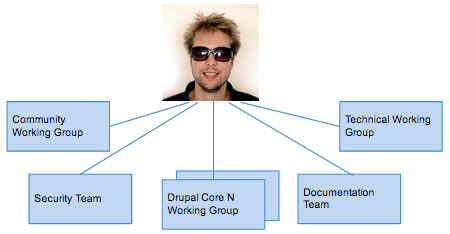
\includegraphics[width=\textwidth,center]{drupal-project-governance-2013.png}

\end{frame}

\section{Teams}

\begin{frame}[allowframebreaks]
\frametitle{Leaders}
\begin{itemize}
\item Heterogeneous and flat organization.
\item \textbf{Drupal Core}: 
\begin{itemize}
\item {Project leader}: Dries Buytaert.
\item {Main releases maintaners}: 
\begin{itemize}
\item {Drupal 6}: G\'abor Hojksy
\item {Drupal 7}: Angela Byron
\item {Drupal 8}: Nathaniel Catchpole
\end{itemize}
\item {Mission}: Help on death-lock issues. Decission making.
\item {\textbf{Slackers}}: The real work is done by contributors and collaborators.
\end{itemize}
\end{itemize}
\end{frame}

\section{Teams}

\begin{frame}[allowframebreaks]
\frametitle{Drupal Contrib}

\begin{itemize}
\item \textbf{Drupal Contributors}: 
\begin{itemize}
\item {+12000 (2011)}
\item {Real Task Force}
\item {Very flat organization}
\item {\textbf{Maintainers}}: The ``official'' scheme, identifying responsabilities for different functionalities:
\begin{itemize}
\item {Branch Maintainers}: ``Project leader as branch maintainer''.
\item {Component Maintainers}: Ajax, Cache, Database, Core, etc.
\item {Topic Coordinators}: Accesibility, Documentation, Security, Translations, User Experience.
\item {Module Maintainers}: Contact module, Dashboard module, Search module.
\item {Theme Maintainers}: Bartik theme, Garland theme, etc.
\end{itemize}
\end{itemize}
\end{itemize}

\end{frame}

\begin{frame}[allowframebreaks]
\frametitle{Drupal Association}

\begin{itemize}
\item \textbf{Drupal Association}: Non-profit Drupal Community Building Association
\item \textbf{Board of Directors: Selected by election}: But who are they in the end?:
Dries Buytaert, President; Angela Byron, Secretary; ...
In the end, important technical people.
\item \textbf{Mission}:
\begin{itemize}
\item Funding, donations achieving
\item Infrastructure status
\item Education and Promotion
\item Ensure DrupalCon celebration
\item Licensing Issues
\end{itemize}
\item \textbf{Non-technical mission}: Do not control CORE/Contrib.
\item \textbf{Staff}: community members, supporting partners, sponsorships.
\end{itemize}
\end{frame}

\begin{frame}[allowframebreaks]
\frametitle{drupal.org}

\begin{itemize}
\item \textbf{Flat organization}: Somehow, mixed and mingled. At least, it is documented.
\item \textbf{Different and heterogeneous roles}, such as:
\begin{itemize}
\item{Sysadmins}
\item{Issue Tracking}
\item{Downloads}
\item{Groups}
\item{Documentation}
\item{Version Control/Git}
\item{QA (Quality Assurance)}
\item{CI (Continuous Integration, via Jenkins)}
\item{Security}
\item{DrupalCon Websites}
\end{itemize}
\end{itemize}
\end{frame}

\section{Interaction}
\begin{frame}[allowframebreaks]
\frametitle{Interaction}
\begin{itemize}
\item{"No special rules"}: Everybody can communicate to anybody, with some logic, and keeping the code of conduct.
\item{"Core Office Hours"}: Mentorship.
Tuesday: 12.am - 2.pm (Eastern)
Wednesday: 12.am - 2.pm (Eastern)
\item{"Change proposals"}: Can be performed by anyone:
\begin{enumerate}
\item Propose your idea (IRC, Twitter, groups.drupal.org, Drupal Planet, etc).
\item Propose a patch
\item The action: Normally occurs on the Issue queue. 
\end{enumerate}
\item{"Bug reporting"}: Can be performed by anyone. A possible workflow:
\begin{enumerate}
\item{User}: Bug posting to Bug issue queue
\item{Programmer}: Fix -> Needs Review
\item{Tester}: Test: -> Fix, OK.
\end{enumerate}
\end{itemize}
\end{frame}

\begin{frame}[allowframebreaks]
\frametitle{Interaction}
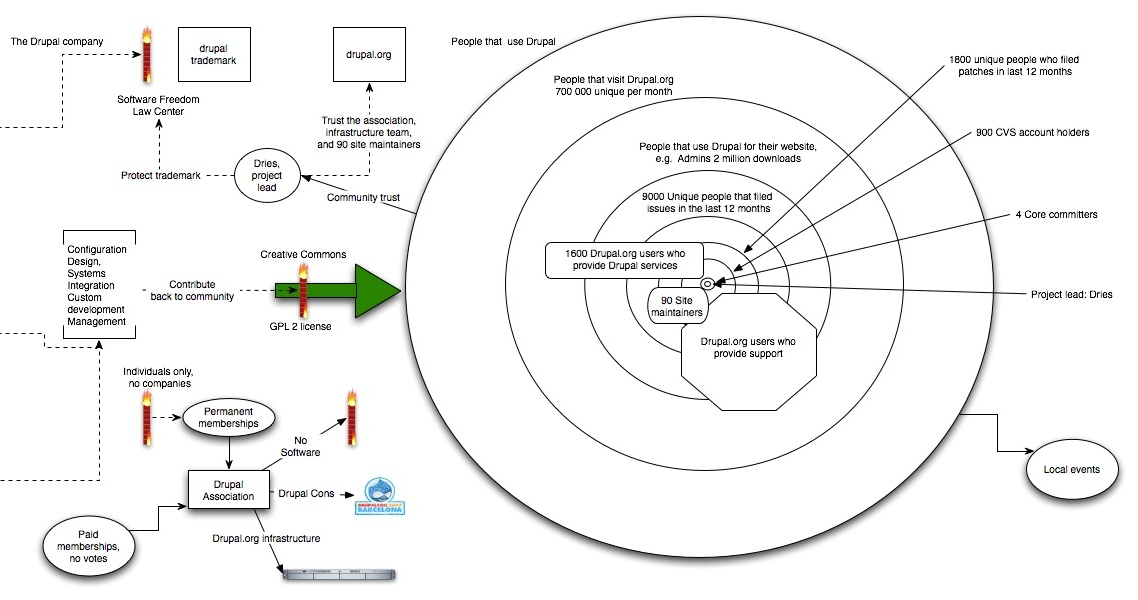
\includegraphics[width=340pt]{organization00.jpg}
\end{frame}

\section{Social}
% 
\begin{frame}[allowframebreaks]
\frametitle{Reference Conference}

\begin{itemize}
\item \textbf{DrupalCon}: Reference Conference for Drupal Community
\item \textbf{Start}: 2005: Belgium. 70 people.
\item \textbf{When?}: Normally, twice a year (1 in Europe, 1 in States). Some execptions (2013: Sydney, Portland, Prague)
\item \textbf{2011}: 3000 people: Showing how the community has grown up.
\item \textbf{2013}: 1840 tickets sold (2000 participants?). Biggest in Europe.
\end{itemize}

\end{frame}

\begin{frame}[allowframebreaks]
\frametitle{DrupalCon Main Goals and Activities}

\begin{itemize}
\item \textbf{Community Building}: Growing and strengthen .
\item \textbf{Promotion}: Marketing and Project acceleration.
\item \textbf{Revenues}: For community programs. Portland DrupalCon: +970000\$.
\item \textbf{Success}:  measured in:
\begin{itemize}
\item Attendees, Cx0 attendees, Students in training.
\item Speakers.
\item After hour events (community building).
\end{itemize}
\end{itemize}

\end{frame}

\begin{frame}[allowframebreaks]
\frametitle{Other social interaction}
\begin{itemize}
\item \textbf{User Group Meetups}: Informal meetups (having a beer, small audience talks, etc.)
\item \textbf{Drupal Camps}: All over the world. Small conferences (75 to 300 people). "Mini-DrupalCons".
\item \textbf{Code Sprints}: Like hackatons: normally weekends. No lessons. Features coding, Bug killing, etc.
\end{itemize}

\end{frame}

\section{Conclusions}
\begin{frame}[allowframebreaks]
\frametitle{Conclusions}

\begin{itemize}
	\item Open development model producing cutting-edge platform
	\item Contributors have a stronger voice in the project and greater influence on the future of Drupal
	\item In the end, there exists a benevolent dictator in the project
	\item Flat organization, somehow a Cathedral of Bazaars
	\item Growing community, close social interaction
	\item DrupalCon: Reference Conference. Successful and profitable
\end{itemize}

\end{frame}

\section{Question}
\begin{frame}[allowframebreaks]
\frametitle{Questions}

\Huge{QUESTIONS?}

\end{frame}

\begin{frame}
\frametitle{References}

% Just for format reference

\begin{itemize}
\tiny{
\item Angela Byron, Drupal 7 maintainer, ``Drupal Community Demystified''
 \url{http://www.youtube.com/watch?v=PSjkRJ2mM54}

\item Stephanie Torres, ``Drupal Association Board Meeting''
 \url{https://association.drupal.org/node/18208}

\item Drupal Maintainers
 \url{https://api.drupal.org/api/drupal/MAINTAINERS.txt}

\item DrupalCon
 \url{https://drupal.org/drupalcon}

} %tiny
\end{itemize}

\end{frame}


\end{document}
